\documentclass{bioinfo}
\copyrightyear{2015}
\pubyear{2015}

%%% SETTINGS %%%
\usepackage{tikz} %ticks in tables
\def\checkmark{\tikz\fill[scale=0.3](0,.35) -- (.25,0) -- (1,.7) -- (.25,.15) -- cycle;}
\usepackage{listings} %code format
\usepackage{color}
\definecolor{lightgray}{rgb}{.9,.9,.9}
\definecolor{darkgray}{rgb}{.4,.4,.4}
\definecolor{purple}{rgb}{0.65, 0.12, 0.82}
\definecolor{darkgreen}{rgb}{0.0, 0.2, 0.0}

\lstdefinelanguage{JavaScript}{
  keywords={break, case, catch, continue, debugger, default, delete, do, else, false, finally, for, function, if, in, instanceof, new, null, return, switch, this, throw, true, try, typeof, var, void, while, with, attr, text, select},
  morecomment=[l]{//},
  morecomment=[s]{/*}{*/},
  morestring=[b]',
  morestring=[b]",
  ndkeywords={class, export, boolean, throw, implements, import, this, D3, append},
  keywordstyle=\color{blue}\bfseries,
  ndkeywordstyle=\color{red}\bfseries,
  identifierstyle=\color{black},
  commentstyle=\color{purple}, %commentstyle=\color{purple}\ttfamily,
  stringstyle=\color{darkgreen}, %stringstyle=\color{darkgreen}\ttfamily,
  sensitive=true
}

\lstset{
   language=JavaScript,
   backgroundcolor=\color{lightgray},
   frame=single,
   extendedchars=true,
   basicstyle=\footnotesize\ttfamily,
   showstringspaces=false,
   showspaces=false,
   numbers=left,
   numberstyle=\footnotesize, % numberstyle=\footnotesize\color{lightgray},
   numbersep=5pt,
   tabsize=2,
   breaklines=true,
   showtabs=false,
   captionpos=b
}


%%% DOCUMENT %%%
\begin{document}
\firstpage{1}

\title[short Title]{Data visualization using D3}
\author[Data visualization using D3]{Jes\'us Alejandro Vald\'es Vald\'es, and Philipp M\"uller}
\address{}
\history{}
\editor{}

\maketitle

\begin{abstract}
\section{Motivation}
\newline
Long before people started to collect data in a digital format, they depended on visual representations of data.
One of the earliest devices to visualize the abstract concepts of the numerical system and basic arithmatic was the Abacus (figure \ref{fig:abacus}). %\citep{wiki:abacus}.
Numbers are represented by small spheres on a wire, shifting them from left to right you can add or subtract values and count the remaining balls.
This simple visualization of the numerical system and basic arithmatic is still used today in pre-schools and elementary schools, because visualizations convey information in an universal manner and make it simple to share and communicate ideas with others.
\newline
As huge amounts of data are collected nowadays, data visualization software becomes more and more important. A visual representation enables us to find relevance of millions of variables, communicate concepts and even predict future behavior based on patterns.
\newline
In our report we will discuss different visualization methods for data in a web based context, available JavaScript libraries, why we decided to use D3.js, and explain the core concepts of D3.

\begin{figure}[!tpb]
\centerline{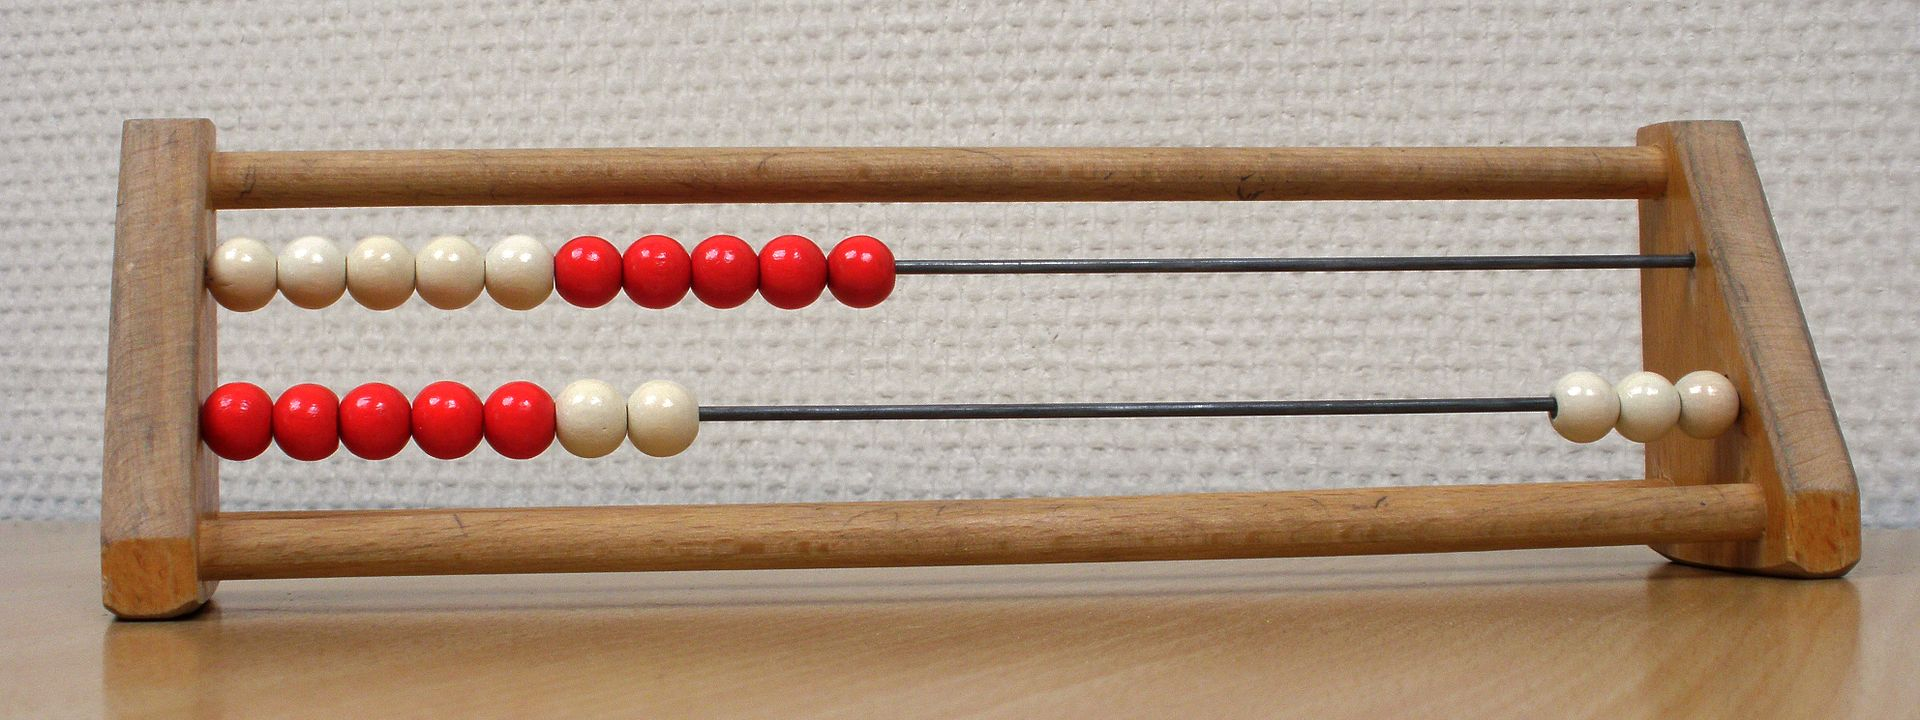
\includegraphics[width=70mm]{abacus.jpg}}
\caption{Simple abacus}\label{fig:abacus}
\end{figure}

\section{Availability}
\newline
D3.js is a free JavaScript library which can also be customized according to your own needs. Further information how to download or link it can be found on their official website d3js.org.

\section{Contacts}
\newline
Jes\'us Alejandro Vald\'es Vald\'es: alejandro.valdesval@gmail.com \newline
Philipp M\"uller: philipp.mueller@tum.de
\end{abstract}

\section{Introduction}
\subsection{How can we visualize data in a browser}
Before we move on which libraries exist to represent data in web browsers we first have to talk about the different approaches generally used to draw in browsers.
There are three common approaches to draw data in modern web browsers, they are:
\begin{enumerate}
\item HTML elements
\item Canvas
\item SVG
\end{enumerate}

% HMTL ELEMENTS
\textbf{HMTL elements} can be styled to represent data. For example a div could be used with different width, height and color style parameters to represent a bar in a bar chart.
However building a framework solely on HTML elements and styling them is clunky and does not scale well.
The reason why it doesn't scale well is that complex or round shapes are hard to portray with HTML elements and come with performance issues. These issues are the result of hundreds or thousands tiny HMTL elements you need to create and draw to be able to represent complex shapes.
On the other side a big advantage of HTML elements is that they are supported in every browser.
They also provide the same functionalities as DOM elements, such as events and other behavior.
Another advantage of DOM elements is that they can be styled with CSS (Cascading Style Sheet) files.
\newline
% CANVAS
\textbf{Canvas} is a HMTL5 element and can be seen as a drawable Bitmap surface.
It provides different drawing methods that enable the visualization of any shape.
Canvas however doesn't have any knowledge about the drawn objects, it only draws pixels.
This means that there are no predefined event callbacks per element that we are used to from DOM elements.
Another feature of Canvas, that might be problematic, is that Canvas redraws the visualization with a fixed update rate. Which might put unnecessary strain on our computational resources.
The browser support for Canvas can be found in table \ref{t:support} for the main browsers. The lowest browser version that supports all baisc features of Canvas  is listed.
\newline
% SVG
\textbf{SVG} is also a HTML5 element and defines a scriptable drawing surface. SVG stands for Scalable Vector Graphic, which implies that it's resolution independent. In this case resolution independence means that, independently of your zoom level, round shapes will stay round and won't get pixelated. 
It also provides drawable elements that can be modified by property parameters to visualize any shape needed. In contrast to Canvas, SVG elements are DOM elements, this means we can easily define event callbacks on them. SVG also provides simple functions to animate elements.
The support for SVG for the main browsers can also be found in table \ref{t:support}.

\begin{table}
\begin{tabular}{ l | c | c | c | c | c } 
		& Chrome & Internet Explorer & Firefox & Safari & Opera \\
\hline
Canvas	& 4.0 & 9.0 & 2.0 &	3.1 & 9.0 \\
SVG		& 4.0 & 9.0 & 3.0 &	3.2 & 10.1 \\
\end{tabular}
\caption{Support table for Canvas and SVG, only the lowest browser versions are listed that fully support all features.} \label{t:support}
\end{table}

In comparison Canvas has a better performance than SVG if a big amount of elements (approximately more than thousand) have to be drawn.
For our project we decided to use SVG over Canvas, because we wanted to create an interactive data visualization with only a small number of elements. As mentioned before, it is very easy to define callback functions for different events such as mouse click or hover events on SVG elements. This helps us to create a more interactive web application in less time.

\subsection{Data visualization libraries}
There is a huge amount of data visualization libraries available online.
But because of limited time, only a few were selected for a closer inspection. 
The selection criteria were mainly the size of the community, the support, dependencies and documentation.
The documentation and also availability of tutorials were of special importance, because everything was learned from scratch in a limited time.
The table \ref{t:libs} shows a small selection of libraries that mostly or completely satisfied our criteria.

\begin{table}
\begin{tabular}{ l | c | c | c }
Library 			& SVG			& Canvas 		& HTML elements \\
\hline
D3.js				& \checkmark 	& \checkmark 	& \checkmark 	\\
Raph\"ael.js		& \checkmark 	& \textbf{-}	& \textbf{-}	\\
vis.js 				& \checkmark 	& \checkmark 	& \checkmark 	\\
Paper.js			& \textbf{-}	& \checkmark 	& \textbf{-}	\\
Chart.js			& \textbf{-}	& \checkmark 	& \textbf{-}	\\
and many more 		& \vdots 		& \vdots 		& \vdots 		\\
%\hline  
\end{tabular}
\caption{Small selection of available JavaScript data visualization libraries and their base method} \label{t:libs}
\end{table}

% D3.JS
It's important to note that \textbf{D3.js} is a general purpose visualization JavaScript library. It is used for manipulating data bases documents without being linked with a proprietary framework.
That simply means that you don't have to learn a new visualization language or syntax if you already know SVG or Canvas.
\newline
% RAPHAEL.JS
The library \textbf{Raph\"ael.js} uses the SVG WC3 recommendation and VML (Vector Markup Language) to create graphics. This enables Raph\"ael to be compatible with older browsers as well as modern browsers.
\newline
% VIS.JS
The \textbf{vis.js} library uses different visualization methods, depending on the called function, to create a certain representation.
\newline
% CHART.JS
The \textbf{Chart.js} library uses the HTML5 Canvas element, but also provides polyfills in order to support older browers like Internet Explorer 7.
\newline
% PAPER.JS
The Paper.js library uses the HTML5 Canvas element to draw data.
\newline
% WHY D3?
For our application it was decided to use D3.js, because it has a good, active and big community as well as an excellent documentation with a variety of great examples.
Many well written tutorials from community members and other external sources can be easily found, this helped in the understanding of D3's core concepts and their practical application.
Another important criteria in our case was time. Developing an attractive interactive web application with D3 in conjunction with SVG is very easy and very fast, because SVG elements are DOM elements and D3 binds data to DOM elements. More on this subject in the following section \ref{s:d3}.



\section{D3 - Data Driven Documents} \label{s:d3}
As mentioned before, one of the most important libraries for data visualization and the main topic of this paper is the JavaScript library D3. The name D3 stands for Data Driven Documents and its main function is to bind data to DOM elements with the goal of creating stunning interactive data oriented visualizations suitable for the web.
\newline
Before diving into the core concepts of D3, a brief history of D3 will be presented.
D3 was developed in the year 2011, mainly by Mike Bostock and Jeffrey Heer, which were also the developers for D3s predecessor Protovis.
\newline
Protovis was developed in the year 2009 amid a growing necessity for new technologies capable of creating visual content for the web. Protovis owned its success to the fact that it was a Plugin-less library. Plugin-less means that it didn’t need a plugin to work while most of the other visualization libraries strictly needed one. Protovis was designed to be accessible to non-programmers as it was a learn by example library.
That design concept was also kept for D3.

\subsection{Loading of external data}
It was previously stated that D3 stands for Data Driven Documents, but: What exactly is data and how can a developer obtain it? Data is a collection of information used for analysis. The easiest way of representing data using JavaScript is through the use of a variable, of course a developer can also opt for more powerful data structures, such as an array, a matrix or even objects and arrays of objects. This and the use of D3 enables the developer to create simple static data visualizations, or visualizations via user input. A more useful way of retrieving  data for D3 is from a file or through an API call, luckily D3 provides methods to do exactly that.
Importing data is often used in combination with API's and databases. Therefore a change in the backend system will result in an updated visualization without any additional programming effort.
Using for example the csv, html, json, tsv, xml or xhr methods a developer could obtain data from different sources.

\subsection{Selections}
After a developer has found suitable data for his work, he now needs a way of binding said data to a selection of DOM elements, so that it can be visualized on a website. 
To do this D3 provides a selection type which is a subtype of JavaScripts arrays and extends their functionality. 
D3 selections can be acquired with the select() and selectAll() methods. These methods will return an array of DOM elements from the current document.
\begin{lstlisting}
var selection = d3.selectAll("p");
\end{lstlisting}
In this small code example the selection will contain every paragraph in our current document. The selection is obtained via the selectAll() method with the filter parameter for parapraph DOM elements.
Selections in D3 use CSS3 selectors to select elements which means that you can select DOM elements the following ways:
\begin{itemize}
\item Tag ("div")
\item Class (".myClass")
\item Id ("\#thisID")
\item Attributes ("[color=red]")
\item Logical AND (".this.that")
\item Logical OR (".this, .that")
\end{itemize}
Once a selection is retrieved, operators can be applied to modify it in different ways. For example, set or get attributes, styles, properties, HTML and text content. The most powerful thing to do with a selection is to join it to a data set, this will be thoroughly  described in section \ref{s:joins} about joins.
This approach allows us to operate on entire selections at once and therefore "for loops" are rarely needed. D3 also allows method chaining on its selections which makes code more readable and understandable. This looks like the next code snippet:
\begin{lstlisting}
D3.select("body")
	.append("div")
	.attr("class","divClass")
	.append("p")
		.text("I am a paragraph")
		.attr("class","pClass");
\end{lstlisting}
This code first selects our body element then it adds a div element to it, from this moment on the following methods will act on the new div element, so the new class name attribute will only modify our div element and not our body element. The code will then add a paragraph element inside the div, and as before the following methods will only affect our newly appended p element. 
Because selections are based on DOM elements the attribute, style and text method calls on selections will also return the current self reference to the selection of DOM elements.

\subsection{Joins} \label{s:joins}
D3s main goal is to visualize data. Since different ways how to obtain data and how D3 selections of DOM elements have been described, the concept of D3s data join can now be discussed. Joins make D3 a powerfull library and it's an important step in the visualization of data, they are made using the \textit{.data([values[, key]])} method.
This method joins data, specified in values, with the selection the method is called upon, it returns a selection again. What this returned selection contains will be explained in the following section.
\newline
The value parameter can either be specified as an array containing any kind of information or a function that returns an array.
The key parameter is optional and specifies a custom compare callback function.
This function will be used to join selection elements and data elements.
The following code example shows a simplification how the join could look like:
\begin{lstlisting}
for(var i=0; i<data.length; i++) {
	for(var j=0; j<selection.length; j++) {
		if(key(data[i]) === key(selection[j])) {
			// match found! Resulting pair is data[i] and selection[j]
		}
	}
}

function key(d) {
	return d.comparedProperty;
}
\end{lstlisting}
If no function is defined as key parameter D3 will revert to the default function that joins selection elements and data based on their indices.
A simplified join function could look like the following code:
\begin{lstlisting}
// pseudocode
for(var i=0; i<data.length; i++) {
	for(var j=0; j<selection.length; j++) {
		if(i === j) {
			// match found! Resulting pair is data[i] and selection[j]
		}
	}
}
\end{lstlisting}

\subsection{The Update, Enter, and Exit sub selections}
In this section the figure \ref{fig:venn} shows a venn diagram which might help you understand the following explanation better.
The circle with the label \textit{Elements} represents all DOM elements of our selection. The selection on the other hand represents the current state of our document.
The data values are the circle with the label \textit{Data}.
Because we want our document state to be driven by our data values, we have to compare them. 
In order to compare the current state (selection) with our wanted state (data values) we perform the join operator.
When we join data on a selection D3 provides us with three different sub selections as seen in figure \ref{fig:venn}.
These sub selections can be defined as:
\begin{enumerate}
\item The \textbf{update} sub selection is obtained by calling the \textit{data(values)} operator on a selection. This operator will also save the other two sub selections as references in the update sub selection.
The update sub selection contains all elements for which there exists matching data.
\begin{lstlisting}
var updateSubSelection = d3.select("svg").selectAll("rect").data([values]);
\end{lstlisting}
In this example we join our data values on a selection that contains all rectangles in the first SVG element we find in our current document.

\item The \textbf{enter} sub selection can be accessed by calling the operator \textit{enter()} on the update sub selection.
The enter sub selection contains all data values that did not find a match in our currently displayed selection of elements. We can initialize the data sub selection by appending to it. Otherwise changes to the sub selection won't persist.
\begin{lstlisting}
var enterSubSelection = updateSubSelection.enter().append("rect");
\end{lstlisting}
As mentioned before, in order to add the data to our document we have to add DOM elements containing our data into the document. In this example we used the append method to do so.
Interesting to note here is that after calling the append operator the variable updateSubSelection will also contain our enterSubSelection.
Therefore we must be careful in what order we call our operators on the update and enter sub selections.

\item The exit sub selection can be accessed by calling the operator \textit{exit()} on the update sub selection.
The exit sub selection contains all elements of the selection that did not find a match in the data values.
Often we want to remove those elements from the document. This can be done via remove call on the exit sub selection as shown in the following example:
\begin{lstlisting}
var exitSubSelection = selection.exit();
exitSubSelection.remove();
\end{lstlisting}
\end{enumerate}

This seperation of the join into three disjunctive sets allows us to specify precisely what operations have to be run on which selections. Due to its disjunktive natur this can also improve the performance because we don't have to handle all sub selections, but pick the sub selections we are interested in.
Which brings us back to the meaning of D3, Data Driven Documents.
As we have seen we can transform documents based on data, e.g. the creation and destruction of DOM elements by calling operators on sub selections, which we obtain via data joins on selections.
We can also modify them by calling different available operators such as .attr(), .style() and .text() on selections.
Changes in those selections can be animated via the .transition() operator that we will discuss in the section \ref{s:transitions}.

\begin{figure}[!tpb]
\centerline{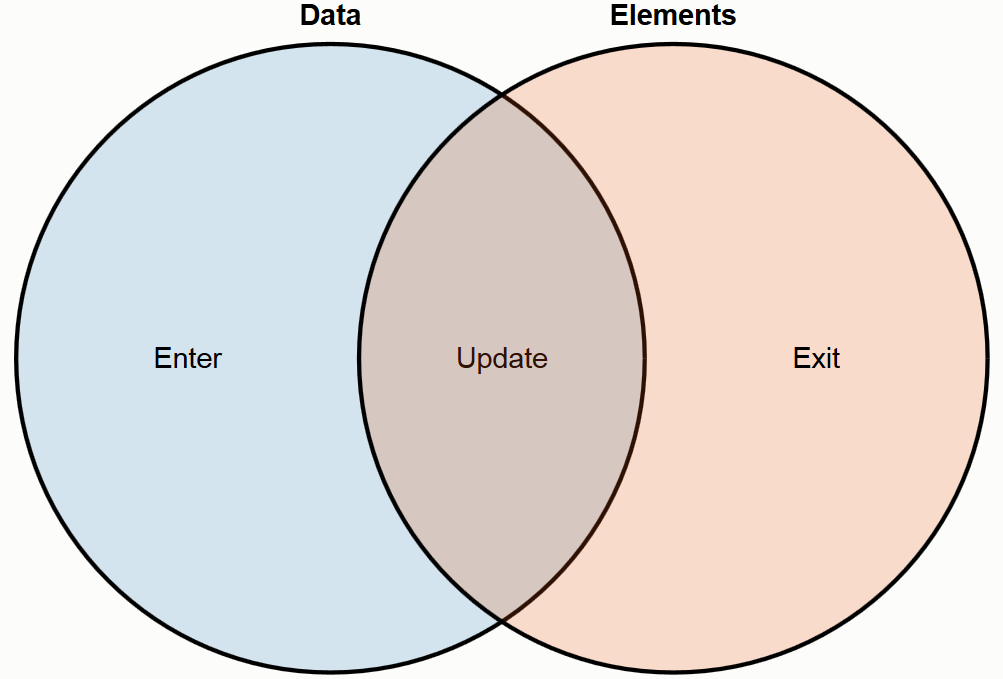
\includegraphics[width=70mm]{vennDiagram.PNG}} %TODO reference to mike bostocks blog
\caption{Venn diagram}\label{fig:venn}
\end{figure}


\subsection{Dynamic properties}
As mentioned in the previous section D3 enables us to modify selections dynamically.
The syntax has many similarities with jQuery, however there exists a big difference.
Properties such as stlyles, attributes and text can not only be specified as a constant but also as a function of data, and the index associated with the element that calls the method.
To better understand this concept the following example shows how we can use dynamic properties.
In the next code snippet we set the name and font size of each paragraph to a constant variable.
We assume that there exists at least three paragraphs in our HTML body.
\begin{lstlisting}
d3.select("body").selectAll("p")
    .text("See")
    .style("font-size", "8px");
\end{lstlisting}
This however might not be what we want. 
If we want to set the name of each paragraph to a different value and also increase the font size with increasing indice of the paragraph, the code could look something like this:
\begin{lstlisting}
d3.select("body").selectAll("p")
    .data(["See", "The", "World"])
    .text(function(d) { return d; })
    .style("font-size", function(d,i) { return (i*4+8) + "px"; });
\end{lstlisting}
Here we join the selection with data values which represents our paragraph names. Further we call our text and style operators on the update sub selection that will contain all three paragraph elements, because we join based on array indices.
As you can see the operators have a function defined in them. If you define a function D3 will pass this function the self reference of the element (this), the associated data value as first parameter and the global index of the element in the array as second parameter. Both parameters are optional. 
Based on those informations we define for example the font size in the style property by the base value of 8 pixels plus four times the index of the element.


\subsection{Transitions} \label{s:transitions}
In the previous sections we have seen how a developer could select an element and change its attributes, however these changes would take place immediately. To create a more interactive and responsive application we also want to have animations. Luckily D3 provides transitions that enable us to apply these exact changes over time via interpolation, thus achieving an animation effect. The transitions have the following life cycle:
\begin{enumerate}
\item The transition is scheduled. (Gets schedule with selection.transition() call in JS)
\item The transition starts. (After the delay, if delay was specified)
\item The transition runs.
\item The transition ends
\end{enumerate}
It is important to notice that transitions are exclusive and only act one given element, so only one transition can be executed at a given time, any new transitions will immediately stop any transitions that were running.
You can also define custom interpolation functions for transitions, they have to take a parameter $t \in [0,1]$.

\subsection{Our web application - See the world}
To demonstrate a small portion of the power of D3, we developed a small web application that would allow us to get a feeling of the core concepts of D3 and what it means to work with it. The application is called “See the World” and it's meant to be used to create social conscience for the difference between countries. Using an interactive map users can select any country in the world and click on it to see a grahpical representation of  how many citizens out of 100 have internet access, and the average yearly income per capita.
\newline
All of the visual elements were created with HMTL5 SVG and D3. The data gets pulled from the world bank API, which means an internet connection is required. To see the source code or simply check out the application, go to https://github.com/PhilippMueller1991/JS-Visualization

\subsection{Discussion}
\subsubsection{Disadvantages of D3}
\hfill \break
D3 is a very powerful library however it does have its disadvantages. For example, it has a steep learning curve and as it is largely used with SVG elements one could say that it is not IE8 compatible (because of SVG).
D3 can be used to create charts, but it is not a graphing library, the user should not expect really easy out of the box methods that would do all of the work, such as makePieChart(50,50), D3 requires more work than that. Another big disadvantage is that, because it works with the DOM, response time can become problem on very large documents.

\subsubsection{Advantages of D3}
\hfill \break
However D3 also has a lot of advantages. One advatage is that it has a great community and that because it is not a graphing nor a charting library it gives the user total creative freedom to visualize whatever they want, however they want. Other advantages are that it uses commonly known selectors.
D3s capabilities to animate selections via transitions is also a advantage.
D3 in combination with SVG also results in fast development cycle and empowers users to protoype ideas very fast.


\section{Conclusion}
Throughout this report we have learned about one of the biggest visualization library for JavaScript which in the last couple of years has been used by data visualization programmer and experts all over the world to represent data in ways that break past barriers of simple charts and plots.
We have learned about the backbone of D3 and how it allows us not only to create static content, but also dynamic real time applications. With the help of its great community and documentation, anyone with some previous JavaScript knowledge can start creating his or her own visualizations, that is if they dedicate enough time to invest some time to overcome the steep learning curve.

To finish this report it is necessary to point out in which cases it would be better to opt for other technologies.

\subsection{When not to use D3}
\begin{enumerate}
\item If you have no time to learn new concepts
\item If advanced big data operations are needed, however D3 can be combined with another library to neutralize this disadvantage.
\item Real graphing software is needed and you don't total control over creative aspect of graphs. You just want some graphs really fast with nearly no effort. 
\end{enumerate}

\subsection{When to use D3} 
\begin{enumerate}
\item If you want is a Plugin-less visualization library. Which means it does not require any other libraries to work. You don't have to worry about other libraries creeping in your application like it is often the case with libraries that are based on jQuery.
\item If you want the visualization not be bound on any specific visualization framework or HTML5 element such as Canvas or SVG.
\item If you want total creative freedom.
\item If you want to quickly develope a prototype.
\end{enumerate}

\end{document}
